\documentclass[12pt]{ociamthesis}

\usepackage{amssymb}
\usepackage[utf8]{inputenc}
\usepackage{polski}
\usepackage{url}
\usepackage[hidelinks]{hyperref}
\usepackage[table,xcdraw]{xcolor}
\hypersetup{
	pdftitle={Uczenie głębokie i maszynowe a mózg},
	pdfsubject={Praca licencjacka},
	pdfauthor={Mateusz Piotr Moruś},
	pdfkeywords={}
}
\usepackage{graphicx}

\graphicspath{ {./Images/} }
\AtBeginDocument{\let\textlabel\label}

% Make the numbering of figures continuous
\counterwithout{figure}{chapter}
% Make the numbering of tables continuous
\counterwithout{table}{chapter}

\title{Uczenie głębokie i maszynowe a mózg}
\engtitle{Deep and machine learning and the brain}
\author{Mateusz Piotr Moruś}
\albumnumber{292540}
\university{Uniwersytet Marii Curie-Skłodowskiej w Lublinie}
\college{Wydział Filozofii i Socjologii}
\field{Kognitywistyka}
\speciality{-}
\submittedtext{Praca licencjacka}
\department{Katedrze Neuroinformatyki i Inżynierii Biomedycznej}
\promoter{dr. hab. Grzegorza Marcina Wójcika, prof. UMCS}
\degreedate{Lublin rok 2021}

\begin{document}

% This baselineskip gives sufficient line spacing for an examiner to easily markup the thesis with comments
\baselineskip=18pt plus1pt

% Set the number of sectioning levels that get number and appear in the contents
\setcounter{secnumdepth}{3}
\setcounter{tocdepth}{3}

% Add a title page
\maketitle

% Add an abstract
\begin{abstract}
	
\end{abstract}

% Start roman page numbering
\begin{romanpages}
	% Generate and include a table of contents
	\tableofcontents
	% Create a group for list of figures and list of tables to fit both on one page
	\begingroup
	\let\clearpage\relax
	% Generate and include a list of figures
	\listoffigures
	% Generate and include a list of tables
	\listoftables
	\endgroup
% End roman page numbering
\end{romanpages}

% Include the introduction
\chapter*{Wstęp}
\addcontentsline{toc}{chapter}{Wstęp}

% Include the first chapter
\chapter{Neuronaukowe korzenie uczenia maszynowego}

Już niedługo po pierwszych teoriach i propozycjach dotyczących maszyn przeprowadzających obliczenia przedstawiły się one jako ciekawa koncepcja dla filozofii umysłu i psychologii.
Maszyna Turinga ze swoimi możliwościami przetwarzania informacji oraz terminologia z nią związana stały się nową popularną metaforą działania umysłu.
Aktualnie prawie każdy większy dział nauk humanistycznych ma swój komputacjonistyczny odłam skupiający się na tym właśnie aspekcie jako wbudowanej cesze świata rzeczywistego.
Był to kolejny z trendów analogii i metafory w psychologii \cite{vroon1987man}, jednak z biegiem czasu przez wielu uważany za coraz bliższy prawdy.

Największą różnicą między możliwościami umysłu człowieka a tym, co w przyszłości zostanie nazwane komputerem była koncepcja uczenia się.
Pierwsze użycie sformułowania "uczenie maszynowe" przypisuje się Arturowi Samuelowi, który takim określeniem opisał algorytmy podejmujące decyzje bez wcześniejszego jawnego zaprogramowania ich do takiego ich wykonywania \cite{koza1996automated}.
Dzisiaj ten dział informatyki obudowuje wiele różnych paradygmatów takich algorytmów.
Najwcześniej używanym były algorytmy genetyczne inspirowane ewolucyjnym charakterem przyrody.

Tak jak psychologia czerpała z informatyki inspirację przy budowaniu metafory komputerowej, tak dziedzina uczenia maszynowego inspirowała się obecnymi w naturze zjawiskami wszelkiego rodzaju uczenia się.
Idea algorytmów genetycznych i programowania genetycznego została wyprowadzona jako przeniesienie teorii ewolucji w naturze.
Najbardziej fundamentalna jednostka popularnych dzisiaj sztucznych sieci neuronowych -- sztuczny neuron, czy perceptron -- zostały po raz pierwszy zaproponowane jako matematyczny model naśladujący działanie neuronu biologicznego \cite{mcculloch1943logical}.

Początkowo neuron McCullocha-Pittsa bezpośrednio odwzorowywał działanie biologicznego odpowiednika, w tym na przykład traktując wyjście modelu binarnie jako \emph{aktywne} lub \emph{nieaktywne}.
Później także podobnie jak w biologicznym układzie nerwowym złożonym ze skomplikowanej sieci neuronów zaczęto wykorzystywać perceptrony wielowarstwowe propagujące sygnał wgłąb modelu \cite{rosenblatt1961principles}.
Mimo tego, że koncepcje podstawowe wykorzystane w sztucznych sieciach neuronowych były bezpośrednio zainspirowane biologicznymi odpowiednikami, szybko okazało się, że wprowadzane modyfikacje architektury i działania sieci znacznie poprawiają ich skuteczność.
Zmiany te jednak nie tylko nie były wynikiem przełożenia wiedzy neuronaukowej do uczenia maszynowego, ale przeciwnie -- odstępowały od podobieństwa do natury na rzecz złożonych modeli matematycznych oraz udogodnień i usprawnień z nich wynikających.
Z czasem jednak zaczęto odchodzić od takiego modelu wyjścia na rzecz funkcji liniowych, a później złożonych nieliniowych, co okazało się znacznie skuteczniejsze i efektywniejsze \cite{sharma2017activation} w rozwiązywaniu problemów poszukiwania minimum funkcji kosztu.
% Liniowe: \cite{minsky2017perceptrons}, nieliniowe: \cite{haykin1994neural}

Dodatkowo od strony neuronauki pokładano nadzieje, że rozwój tych sztucznych systemów wzorowanych na biologicznym układzie nerwowym pozwoli nam w lepszy sposób zrozumieć mózg.
Wiedziano, że znacznie prostsze jest zrozumienie złożonego systemu poprzez zbudowanie go od podstaw niż próby wykorzystania inżynierii wstecznej na danych obserwacyjnych z nim związanych \cite{braitenberg1986vehicles}.

% Include the second chapter
\chapter{Modularny system symboliczny jako model działania mózgu}

% \section{Modelowanie mózgu}

\section{Kognitywistyczne podstawy i rozwój modelu systemu symbolicznego}
\label{cognitive-basics}
% file:///C:/Users/mmorus/OneDrive/Moje/Studia/Kognitywistyka/Licencjat/References/Computational%20Foundations%20of%20Natural%20Intelligence.pdf

\subsection{Koneksjonizm}

Jedną z pierwszych teorii wiązanych z mózgiem jako systemem symbolicznym był koneksjonizm.
Wyjaśnia on poznanie jako proces wynurzający się ze wzajemnego działania i współpracy pomiędzy podstawowymi elementami przetwarzającymi \cite{bechtel1993case}.

Jest on istotny w ramach omawianego aspektu, gdyż był podstawą teoretyczną abstrakcji działania mózgowych połączeń neuronalnych, która finalnie doprowadziła do pierwszych modeli sztucznych sieci neuronowych.
Jeszcze sam Alan Turing proponował utworzenie architektury komputerowej opartej na jednostki podobne neuronom \cite{copeland1996alan}.

Koneksjonistyczna idea działania poznania sugeruje, że taka abstrakcja -- mimo, że nie oddaje szczegółów działania biologicznego mózgu -- utrzymuje naturę działania mózgu, funkcje poznawcze.
Jak jednak zostało już opisane i zaznaczone w rozdziale \hyperref[chapter1]{rozdziale \ref*{chapter1}}, szybko okazało się, że takie powiązanie okazuje się być znacznie bardziej skomplikowane i złożone.

\subsection{Kognitywizm}

Na koneksjonistyczne problemy modelowania działania mózgu odpowiada kognitywizm.
W tym podejściu poznanie definiuje się jako manipulację symbolami formalnymi, gdzie wnioskowanie opiera się na manipulacji reprezentacjami symbolicznymi odpowiadającymi informacji o środowisku otrzymanej przez percepcję.
Formalizacją takiego ujęcia była hipoteza systemu symboli fizycznych \cite{newell2007computer}, w której to taki system symboli fizycznych jest jednocześnie niezbędny oraz wystarczający dla inteligentnego zachowania.

Takie podejście okazało się być bardziej zbliżone działaniu mózgu, pomogło w pierwszej fazie uformować się kognitywistyce oraz dało początek niektórym sztucznym architekturom kognitywnym opartym na regułach, takie jak SOAR \cite{laird2019soar}\footnotemark.
\footnotetext{
	Projekt SOAR jest do teraz aktywnie rozwijany.
	Szczegółowe informacje na jego temat znajdują się na oficjalnej stronie: \url{https://soar.eecs.umich.edu}.
	Repozytoria związane z projektem są otwartoźródłowe i znajdują się w serwisie GitHub: \url{https://github.com/SoarGroup}.
}
Ponownie jednak taka architektura okazała się nie oddawać w pełni złożoności działania poznania u człowieka.

\subsection{Modelowanie probabilistyczne}

W ludzkim poznaniu, a co za tym idzie w modelu działania mózgu, informacje czy samo wnioskowanie nie opiera się wyłącznie na Boole'owskiej prawdzie i fałszu, tak, jak ma to miejsce w logice pierwszego stopnia, na której oparte były poprzednie architektury.
Zazwyczaj człowiek nie jest ``pewny'', ale ``przekonany''.
Umysł operuje na zdarzeniach natury indukcyjnej i pewność nigdy nie jest rzeczywiście niepodważalna.
Nie brnąc dalej w filozoficzną tematykę czym jest prawda i fałsz, wydaje się być oczywistym, że człowiek działa raczej na zasadzie prawdopodobieństw i nieokreśloności.

Matematyka jednak również była tutaj w stanie pomóc, jako, że logika probabilistyczna była już dostępna i dobrze rozwinięta.
Architektury modelujące oparte na kwantyfikacji stanu świata w terminach stopnia prawdziwości nazywanej teorią probabilistyczną \cite{jaynes1988does}, zbliżyły się jeszcze bardziej do poznania człowieka i modelowania działania ludzkiego mózgu.
Takie podejście jest podstawą wyjaśniania podejmowania optymalnych decyzji wykonywanych w warunkach niepewności.
Są postulaty wskazujące na to, że na poziomie algorytmicznym mózgi wykorzystują algorytmy wnioskowania przybliżonego (\emph{approximate inference}) \cite{andrieu2003introduction} tak, aby wytwarzać wystarczająco dobre rozwiązania dla szybkiego i oszczędnego podejmowania decyzji.

\subsection{Oddolna emergencja a odgórna abstrakcja}

Jeśli zaczniemy rozważania od odwrotnej strony przy pomocy pytania: ``jaki system sztucznie inteligenty byłby najbliższy działania rzeczywistego, biologicznego mózgu'' szybko dotrzemy do wniosku, że byłaby to jego symulacja.
Taki system oparty by był na \emph{oddolnej emergencji} (\emph{bottom-up emergence}), gdzie zachowania i poznanie symulowanego mózgu wyłoniłoby się z symulacji najprostszych jednostek, neuronów oraz ich środowiska.
Jednak jak twierdzi badacz, który zajmował się symulacją systemów wzgórzowo-korowych u ssaków \cite{izhikevich2008large} Eugene Izhikevich, nawet symulacja sekundy działania całego ludzkiego mózgu nie przyczyniłaby się znacząco do neuronauki \cite{Izhikevich2006why}.
Dodając do tego ogrom skali zadania, jakim jest symulacja ludzkiego mózgu można zrozumieć, dlaczego zwrócono się w stronę alternatywnego podejścia.

Rozwój podejść z kategorii \emph{odgórnej abstrakcji} (\emph{top-down abstraction}) jest obrazowany przez poprzednie tematy z \hyperref[cognitive-basics]{tej sekcji}.
Te algorytmy są obliczeniowo wykonywalne i dzięki temu mają potencjał użytkowy do analiz teoretycznych.
Obiecującym punktem powstałym na wyjściu implementacji założeń teoretycznych w praktyce są sztuczne sieci neuronowe, podstawa nowoczesnego głębokiego uczenia i dużej porcji całego uczenia maszynowego.
Można je wiązać z poziomem biofizycznym -- głównym źródłem porównań przy oddolnej emergencji -- jako abstrakcje biologicznych sieci neuronów opartych na częstotliwości (\emph{rate-based}) \cite{dayan2001theoretical}.
Architektury sieci mogą być wytwarzane w procesie ewolucyjnym, czy algorytmów bazowanych na strategiach ewolucyjnych \cite{real2017large}.
Są zgodne również z modelowaniem probabilistycznym, jak zauważono, algorytmy obliczeniowe powstałe w wyniku uczenia są zbliżone efektywnie do wnioskowania bayesowskiego \cite{gal2016dropout, mandt2017stochastic}.
Są związane nawet z bazą komputacjonistycznego podejścia poprzez ugruntowanie reprezentacji symbolicznych w stanach sensorycznych świata rzeczywistego \cite{harnad1990symbol}.

Użycie koneksjonistycznych sztucznych sieci neuronowych wzbogaconych o architektury i struktury innych modelów systemów przetwarzania symbolicznego wydaje się być najbliżej potencjalnej inteligencji sztucznej.
Nie jest to jednak jednoznaczne z tym, że są także najbliżej odwzorowywania działania mózgu.
Aby móc wyciągać wnioski choćby zbliżone do takowych należy wykazać także podobieństwo w przeciwnym kierunku.

\section{Zestawienie modularności mózgu z modularnością sztucznych systemów symbolicznych}

\subsection{Modularność uczenia maszynowego i systemów symbolicznych}

Nowoczesne architektury rozwiązań pojawiających się w dziedzinie uczenia maszynowego mają dodatkowo cechę wyłaniającą się wraz ze wzrostem złożoności systemów -- modularność.

Jej wartość w uczeniu głębokim oraz szerzej pojętych sieciach neuronowych zauważana była już od dłuższego czasu \cite{schmidt1998modularity}.
Co więcej, istnieją powody by wierzyć, że taka struktura jest w pewnym sensie optymalna.
Gdy klasyfikator nieliniowy o budowie modularnej jest poddawany ``procesowi ewolucji'' poprzez aplikowanie szumu do jego wag wewnętrznych, topologia modularna sieci ewoluuje bez wsparcia reprezentacjonalnego \cite{hoverstad2011noise}.

Analizując jako przykład biliniowe konwolucyjne sieci neuronowe (B-CNN) \cite{lin2015bilinear} taką modularność można wyraźnie dostrzec nawet w jednej jednostce sieciowej.
Składa się ona bowiem z czterech kluczowych komponentów:
\begin{itemize}
	\item Dwóch niezależnych strumieni konwolucyjnych służących jako \emph{ekstraktory cech};
	\item Operatora nakładania biliniowego (bilinear pooling) agregującego wyniki strumieni konwolucyjnych do wektora biliniowego;
	\item Głębokiej sieci neuronowej z gęsto łączonymi warstwami służącej za \emph{klasyfikator}.
\end{itemize}
Można więc stwierdzić, że taka sieć neuronowa jest \emph{modularna}. Składa się z połączonych komponentów (modułów), z których każdy jest wyspecjalizowany do konkretnego zadania.
Dodatkowo można zauważyć naturę tej modularności -- jest ona \emph{hierarchiczna}.
Część sieci odpowiedzialna za ekstrakcję cech obrazu składa się z trzech modułów: dwie sieci konwolucyjne działające niezależnie oraz operator agregujący ich wyniki.

Dodatkowo w wykorzystaniu praktycznym takich czy innych sieci czy rozwiązać uczenia maszynowego pojedynczy system traktuje się właśnie jako moduł, którego zadaniem jest wykonanie wymaganej czynności.
Jest to moduł wyspecjalizowany w tym co robi.
Tak tutaj, w przypadku B-CNN jej zadaniem jest klasyfikacja obrazu.
System, który ją wykorzystuje również może być -- a nawet zazwyczaj jest -- modułem.
Przykładowo możemy wyobrazić sobie funkcję wyszukiwarki za pomocą obrazu, która wykorzystuje moduł B-CNN aby skategoryzować obraz, a następnie inne moduły aby wyszukać obrazy z odpowiedniej kategorii.

Taki sposób działania sztucznych systemów symbolicznych jest dość uniwersalny i nazywa się \emph{hierarchiczną modularnością}.
Jest on nieodłącznym elementem informatyki, pozwala na budowanie bardzo złożonych systemów poprzez enkapsulację funkcjonalności.
Co więcej, już prawie 60 lat temu argumentowano, że każdy złożony system jest zorganizowany w sposób hierarchiczny, niezależnie, czy jest on społeczny (np. system transportowy), czy jest fizycznym systemem symbolicznym czy nawet biologicznym \cite{simon1962architecture}.

\subsection{Modularność mózgu}

O tym, że sieci mózgowe są zorganizowane modularnie wiedziano już od pewnego czasu \cite{bullmore2009complex}.
Jednak dopiero niedawno rozpoczęto badania nad charakterem tej modularności.
Nieco konkretniej, zaczęto badać czy jest ona hierarchiczna, tak, jak przewidywał to Simon względem każdego systemu złożonego \cite{simon1962architecture}.
Jak się okazuje, pierwsze próby wyodrębnienia takiej hierarchii modularnej sieci funkcjonalnych mózgu zakończyły się pozytywnymi wynikami \cite{meunier2009hierarchical}.

Dane z przeprowadzonego badania fMRI przetworzono metodą Louvain do detekcji wspólnot.
Wynikiem takiego przetworzenia był wielowarstwowy graf modułów funkcjonalnych, w którym warstwy odpowiadają hierarchii przynależnościowej pod-modułów do modułów wyższego rzędu.
Analiza wyodrębniła pięć największych obszarów (modułów) najwyższego poziomu, do których dodatkowo można przyporządkować funkcje bazując na znajomości funkcji obszarów mózgowych znajdujących się w obrębie danego modułu.
Podział ten przedstawia \hyperref[tab:modular]{tabela \ref*{tab:modular}}.

\begin{center}
	\begin{table}[ht]
		\begin{tabular}{ | c | c | c | }
			\hline
			\begin{tabular}{@{}c@{}} Moduł \\ (funkcja) \end{tabular} & Liczba węzłów & Liczba pod-modułów \\
			\hline
			\hline
			\begin{tabular}{@{}c@{}} Centralny \\ (sensomotoryczny) \end{tabular} & 239 & 11 \\
			\hline
			\begin{tabular}{@{}c@{}} Ciemieniowo-czołowy \\  (główny/uwagowy) \end{tabular} & 138 & 10 \\
			\hline
			\begin{tabular}{@{}c@{}} Przyśrodkowo-potyliczny \\ (pierwszorzędowy wizualny) \end{tabular} & 132 & 1 \\
			\hline
			\begin{tabular}{@{}c@{}} Boczno-potyliczny \\ (drugorzędowy wizualny) \end{tabular} & 101 & 1 \\
			\hline
			\begin{tabular}{@{}c@{}} Czołowo-skroniowy \\ (symboliczny) \end{tabular} & 89 & 24 \\
			\hline
		\end{tabular}
		\caption{Moduły}
		\label{tab:modular}
	\end{table}
\end{center}

Mimo niewielkiej ilości tych modułów najwyższego rzędu można dostrzeć pewne prawidłowości.
Przynależność do stopnia hierarchii nie jest równoznaczna z wielkością modułu.
Na najwyższym poziomie wyodrębniono osiem obszarów, z czego tylko pięć wspomnianych było wystarczająco złożonych by móc podlegać dalszej analizie.

Największy z nich to moduł centralny, \emph{somatosensomotoryczny}.
Jest on jednocześnie dobrym przykładem, że podział modularny zachowywał właściwości podziału funkcjonalnego także na niższych warstwach hierarchii.
Zawarte w module centralnym kora przyśrodkowa oraz kora boczna znalazły się bowiem w osobnych pod-modułach.
Co więcej -- idąc głębiej, w module drugiego poziomu zawierającego korę boczną obszary przedśrodkowe oraz zaśrodkowe były odseparowane od górnej kory skroniowej.

Moduł ciemieniowo-czołowy, drugi pod względem ilości zawartych w sobie węzłów, obejmował obszary funkcjonalnie odpowiadające części mózgowych \emph{głównej} oraz \emph{uwagowej}.
On wraz z poprzednio wymienionym modułem są stosunkowo zrównoważone.
Posiadają one liczbę pod-modułów, która nie odbiega od normy.
Wśród nich jest niewielka ilość dużych pod-modułów i wiele małych.

Następny co do wielkości moduł przyśrodkowo-potyliczny zawiera w sobie pierwszorzędową korę wzrokową, stąd funkcjonalnie przyporządkowany jest jako moduł \emph{pierwszorzędowy wizualny}.
Jeszcze następny -- obszar boczno-potyliczny -- nazwany został modułem \emph{drugorzędowym wizualnym} z powodów analogicznych do wcześniejszego.
Wymienione zostały przeze mnie razem, gdyż dzielą poza faktem, że funkcjonalnie odnoszą się do obszarów wizualnych, dzielą ze sobą jeszcze jedną istotną cechę -- oba posiadają wyłącznie jeden pod-moduł.

Ostatni moduł najwyższego poziomu z tych wartych analizy, czołowo-skroniowy, został nazwany \emph{symbolicznym}.
Podobnie jak inne, nazwa ta została wyciągnięta z określenia, jakim można by było skategoryzować funkcjonalnie obszary w nim zawarte.
On również wyróżnia się spośród pozostałych, ale w kierunku przeciwnym do modułów wizualnych.
Posiada bardzo dużą liczbę pod-modułów o stosunkowo równej wielkości.

Wspomniane prawidłowości oraz różnice między-modularne tworzą dość spójny obraz modularności hierarchicznej w funkcjonalnych sieciach mózgowych.
Modularność jest wyraźna nawet bazując na samej analizie funkcjonalnej oraz spójności powstałych obszarów, dodatkowo potwierdzone przeprowadzonym przez autorów porównaniem, w którym powstała modularność była wyższa niż dla sieci generowanych losowo.
Hierarchiczność również jest zauważalna i dodatkowo mówi nam dużo o naturze tych wyodrębnionych obszarów funkcjonalnych.
Warte spostrzeżenia jest, że te wnioski są zbieżne z analogicznymi sztucznymi systemami symbolicznymi oraz ich topologią.
Obszary wizualne, podobnie jak wykorzystywane w rozwiązania w systemach widzenia maszynowego opierają się na jednej, wysoce złożonej i ``uniwersalnej'' sieci odpowiedzialnej za wyodrębnienie istotnych informacji z otoczenia.
Obszary symboliczne natomiast składają się z wielu małych, ale wysoce wyspecjalizowanych modułów współpracujących w przetwarzaniu informacji.

% Include the third chapter
\chapter{Powiązania uczenia głębokiego i neuronauki}

Modularność działania mózgu jest bardzo wyraźna i prosta w podparciu.
Dodatkowo, jak się okazuje, jej cechy pozwalają sądzić że bardzo przypomina modularność sztucznych systemów symbolicznych, w szczególności z dziedziny uczenia maszynowego, najczęściej oparte na uczeniu głębokim.
Poza tym, że można doszukać się podobieństw i spójności strukturalnych, aby móc rzeczywiście mówić o tym, że dziedziny uczenia maszynowego (głównie za sprawą uczenia głębokiego) oraz neuronauki wydają się dążyć do ponownego ze sobą powiązania należy wykazać podobieństwa funkcjonalne.
Badacze obu dziedzin stale zauważają nowe ścieżki w różne sposoby łączące je ze sobą.
Uczenie głębokie ponownie skutecznie sugeruje się działaniem mózgu w optymalizacji naszych własnych rozwiązań oraz doszukuje się w takich zapożyczeniach drogi rozwoju uczenia maszynowego \cite{lake2017building}.
W neuronauce coraz częściej okazuje się, że wykorzystanie pojęć bezpośrednio z uczenia głębokiego jest nie tylko pomocne w konceptualizacji i rozumieniu, ale także wydaje się być bardzo blisko danych empirycznych \cite{dayan2001theoretical, doya1999computations}.

\section{Hipotezy w kierunku integracji głębokiego uczenia oraz neuronauki}

Jak zostało opisane w \hyperref[sec:differences]{sekcji \ref*{sec:differences}}, po początkowej obustronnej kooperacji między uczeniem maszynowym oraz neuronauką zaczęły pojawiać się rozbieżności.
Uczenie głębokie skupiło się na ścisłej optymalizacji funkcji kosztu przy stosunkowo jednolitej architekturze.
W neuronauce z kolei to zmienna i złożona architektura, dynamika i systemy mózgowe były w centrum zainteresowania i rozwoju dziedziny.

Jednak nowe technologie w zakresie uczenia maszynowego dają możliwość i nadzieję na ponowne zestawienie ze sobą tych dziedzin.
Zaczęto używać funkcji kosztu znacznie bardziej złożonych i zróżnicowanych warstwami i względem czasu \cite{gulccehre2016knowledge, saxe2013exact};
Pojawiły się architektury ustrukturyzowane, w tym wykorzystujące dedykowane systemy pamięci krótko- i długo-terminowych czy uwagowych (LSTM \cite{chung2014empirical}, adresowane lokacją czy zawartością \cite{graves2014neural} oraz inne).

Takie idee dotychczas pojawiały się ekskluzywnie w uczeniu maszynowym.
W niedawnej pracy badawczej zostały zaproponowane trzy hipotezy odnoszące się do działania mózgu \cite{marblestone2016toward}, które -- jeśli okazałyby się prawdziwe -- mogłyby prowadzić do ponownej integracji dziedzin uczenia maszynowego i neuronauki.

\subsection{Mózg optymalizuje funkcje kosztu}
\label{subsec:brain-optimizes-cost-function}

Jeśli ma się okazać, że rzeczywiście uczenie maszynowe i neuronauka mogą być na drodze ponownej integracji, to przede wszystkim muszą mieć zgodne podstawy strukturalne.
W uczeniu głębokim taką niezaprzeczalną podstawą jest funkcja kosztu i proces jej optymalizacji.
Pierwsza, zasadnicza hipoteza wspomnianej pracy \cite{marblestone2016toward} mówi, że mózg również optymalizuje funkcję kosztu.

Optymalizacja sama w sobie nie jest niczym nowym w ujęciu działania mózgu.
Chociażby wykorzystanie energii przy funkcjach motorycznych jest bliskie optymalnemu \cite{taylor2011does}.
Nie odnosi się to jednak tylko do funkcji wysokiej abstrakcji, rezultaty innych badań potwierdzają, że podstawowe elementy budowy mózgu, które pojawiły się w procesie ewolucji służą optymalizacji wydajności transmisji sygnału \cite{paprocki2020optimizing}.

Mimo to ta sformułowana hipoteza może budzić wątpliwości.
Czym bowiem tak na prawdę miałaby być ta funkcja kosztu i w jaki sposób ta optymalizacja miałaby przebiegać?
W uczeniu maszynowym rolę optymalizacji najczęściej przyjmuje algorytm propagacji wstecznej błędu.
Takie podejście w dosłownym jego znaczeniu jest oczywiście niemożliwe do realizacji w mózgu, wymaga bowiem reprezentacji liczbowych w celu kalkulacji pochodnych tworzących gradient funkcji.
Jednak ta hipoteza opiera się na ogólniejszym pojęciu optymalizacji z dwiema tezami:

\begin{itemize}
	\item Mózg posiada mechanizmy odpowiadające za przydzielanie wyniku (\emph{credit assignment}), która pozwala mu odpowiednio poprawiać właściwości;
	\item Mózg posiada mechanizmy pozwalające mu na dobór odpowiedniej funkcji kosztu lub jej modyfikację.
\end{itemize}

Te dwie tezy stojące za hipotezą, że móżg optymalizuje funkcje kosztu są możliwe do podparcia przez kilka możliwych, różnych od siebie solucji.

Jedna z nich odchodzi od idei mechanizmów optymalizacyjnych opierających się na wykorzystaniu metody gradientu prostego (\emph{gradient descent}) czy przydzielaniu wyników sieci.
Zamiast tego skupia się na możliwości, że wspomniane tezy są realizowane na basie lokalnej samo-organizacji.
Jedną z takich teorii jest, że takie uczenie może mieć miejsce na bazie obwodów ``Zwycięzca bierze wszystko'' (\emph{Winner-Take-All Circuits}) w mechanizmach STDP (\emph{Spike-timing-dependent plasticity}) \cite{kappel2014stdp}.
Takie podejście unika potrzeby wykorzystania algorytmu wielowarstwowej propagacji wstecznej.
Nie trzeba jednak szukać nowych teorii, mechanizm taki jak plastyczność Hebbowska (\emph{Hebbian plasticity}) regulująca aktywności synaptyczne jest dobrze znana i zbadana, w tym bardziej złożone jego wersje, na przykład uwzględniające nieliniowość \cite{brito2016nonlinear}.

Istnieją także inne architektury sztucznych sieci neuronowych, które wykorzystują samo-organizacyjne sposoby uczenia, a co za tym idzie, są teoretycznie aplikowalne w przypadku mózgu.
Dla przykładu echoiczne sieci stanowe (\emph{echo state networks}), w których optymalizacja pojawia się wyłącznie na warstwie wyjściowej, czyniąc ją jednocześnie znacznie prostszą w implementacji bez propagacji wstecznej \cite{jaeger2004harnessing}.

Warto jednak przyjrzeć się także możliwości, że mózg w rzeczywistości w pewien sposób wykorzystuje metodę gradientu prostego.
Jest to najskuteczniejsza forma uczenia głębokich sieci neuronowych, w szczególności o dużych rozmiarach, więc być może częściowo odpowiadają także za niesamowite zdolności uczenia się mózgu.
Jest aktualnie wiele zaproponowanych mechanizmów podobnego uczenia, które byłyby ``biologicznie prawdopodobne''.
Jedną z nich jest wersja wspomnianego STDP, gdzie neurony mają kodować pochodne błędu wymagane przy propagacji wstecznej w różnicach częstotliwości aktywacji (\hyperref[fig:spike-timing-dependent-plasticity]{rysunek \ref*{fig:spike-timing-dependent-plasticity}}) \cite{hinton2016can}.
Efektywnie oznaczałoby to, że mózg wykorzystuje mechanizm propagacji wstecznej.

\begin{figure}[!ht]
	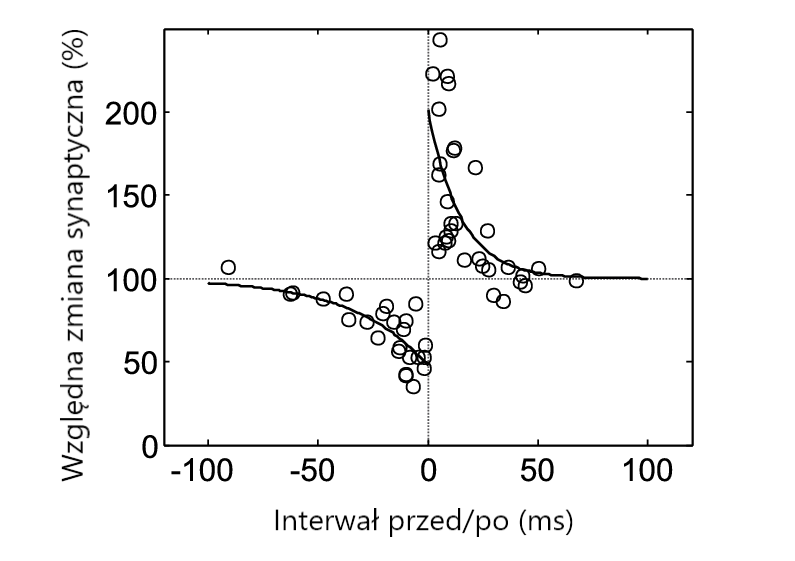
\includegraphics[width=\textwidth]{Images/SpikeTimingDependentPlasticity}
	\caption{Plastyczność zależna od momentu spike'a (STDP)}
	Wykres przedstawia asymetryczne okno czasowe plastyczności zależnej od momentu spike'a (\emph{spike-timing-dependent plasticity}) (źródło: \cite{yao2005synaptic}).
	Jeśli neuron staje się aktywny przed spike'iem pre-synaptycznym, zmiana jest ujemna, a jeśli po - dodatnia.
	Geoffrey Hinton sugeruje, że w ten sposób zakodowana może być pochodna błędu, jako względna zmiana synaptyczna \cite{hinton2016can}.
	\label{fig:spike-timing-dependent-plasticity}
\end{figure}

Asymmetric time window for spike timing-dependent plasticity

Jeśli jednak odstąpimy od metody gradientu prostego, należy skupić się na innych metodach uczenia i optymalizacji.
Mózg posiada kilka mechanizmów, które potencjalnie mogłyby spełniać taką rolę.

Jedno z wyjaśnień opiera się na \emph{kolumnie neuronalnej} (\emph{cortical sheet}), sześciowarstwowej strukturze kory mózgowej, w której każda warstwa odpowiada za wysyłanie sygnałów do określonych obszarów mózgu.
Badacze tworzący modele uczenia w korze przypisują kolumnie neuronalnej rolę uczenia nienadzorowanego poprzez przewidywanie \cite{o2014learning}.
Takie modele budowane są między innymi na bazie przeniesienia konkretnych aspektów neurofizjologii korowej na terminologię komputacjonistyczną, na przykład grupowania hierarchicznego \cite{rodriguez2004derivation}.
Przede wszystkim istotna jest tutaj warstwowość.
Lokalne neurony hamujące skierowane na konkretne części dendrytyczne obszaru neuronów piramidowych L5 mogły by zostać użyte do sprawowania kontroli kiedy i jak odpowiednie sygnały zwrotne i powiązane mechanizmy są używane \cite{marblestone2016toward}.

Innym wyjaśnieniem może być implementacja przez mózg uczenia typu jednego podejścia \emph{one-shot learning}.
Byłoby to zgodne z tym, jak w rzeczywistości często człowiek się uczy.
Wystarczy jedno spostrzeżenie bodźca, który momentalnie zostaje zapamiętany, a nawet może zostać zgeneralizowany do ogólniejszej grupy czy założenia.
Mózg -- zamiast treningu metodą gradientu prostego -- przechowywałby reprezentacje w wagach złożonych sieci komórek gdy obiekty są poddawane transformacjom, podobnie jak ma to miejsce w modelu HMAX (\emph{Hierarchical Model and X}) \cite{serre2007feedforward}.
Dodatkowo mózg miałby potrafić przemieszczać obiekty z pamięci epizodycznej do długotrwałej (w wagach sieci korowej) \cite{ji2007coordinated}.

\subsection{Funkcje kosztu mózgu są zróżnicowane względem obszaru i w czasie}
\label{subsec:cost-function-is-diverse}

Druga hipoteza przedstawiona przez autorów omawianej pracy \cite{marblestone2016toward} opiera się na prawdziwości pierwszej i doprecyzowuje ją: te funkcje kosztu są zróżnicowane względem obszaru mózgu oraz zmienne w czasie.
Trudno sobie wyobrazić, że mogłaby istnieć pojedyncza funkcja kosztu kierująca uczeniem wszystkich sieci funkcjonalnych mózgu biorąc pod uwagę jego modularną budowę opisaną w \hyperref[ch:modularity]{rozdziale \ref*{ch:modularity}}.
Jeśli  ta hipoteza miałaby być poprawna, jak tak funkcja kosztu miałaby być stosowana i jakie fizyczne struktury byłyby do tego wymagane?

Warto zacząć od tego, jakie rodzaje uczenia mogą być wykorzystywane przez struktury mózgowe:

\begin{itemize}
	\item Uczenie nadzorowane w kontekście mózgu może nie wydawać się oczywiste.
	      W końcu jeśli wynik jest znany, jak wymagane jest przy takim typie uczenia, to dlaczego mózg miałby się dalej uczyć?
	      Być może jednak szkolenie opiera się na wykorzystaniu właśnie poznanego poprawnego wyniku w celu lepszej generalizacji.
	      Przykładowo mózg człowieka uczącego się strzelać z łuku może po każdym strzale przechowywać wyniki działania wewnętrznych sieci.
	      Po strzale trafionym różnice między nieudanymi a udaną konfiguracją mogą zostać użyte właśnie do uczenia nadzorowanego.
	\item Uczenie nienadzorowane w kontekście mózgu jest znacznie prostsze do wyjaśnienia.
	      Jest ono bardzo skuteczne w przypadku generalizacji danych z nowej dziedziny.
	      Mogą więc służyć do budowy modeli statystycznych z danych wejściowych, które później z kolei stanowią bardzo dobrą podstawę do innych sposobów uczenia, co czasem nazywa się modelami uprzednio przetrenowanymi (\emph{pre-trained}) i wykorzystywane jest w uczeniu maszynowym \cite{erhan2009difficulty}.
	      Mogą także w przybliżony sposób oceniać cechy świata zewnętrznego, które nie mogą być (lub nie powinny być) empirycznie sprawdzone czy zbadane, np. czy dane zjawisko czy stworzenie powinno się uznać za groźne.
	\item Uczenie przez wzmacnianie mimo wszystko wydaje się być najczęściej wykorzystywane i nawet intuicyjnie najlepiej dopasowane do tego, jak widzimy, że uczy się mózg.
	      Zdecydowana większość działań sprowadza się do wykonania akcji i odebraniu, czy udało się w jej rezultacie uzyskać wynik spodziewany lub oczekiwany lub preferowany, albo odwrotnie, czy nie doprowadziła do negatywnych konsekwencji.
	      W taki sposób uczą się dzieci, w taki sposób uczone są zwierzęta i być może -- na niższym poziomie -- tak uczą się wewnętrzne systemy mózgu człowieka.
\end{itemize}

Dla uczenia nadzorowanego musiałby jednak istnieć system porównawczy, pozwalający na utworzenie wektora błędów, który z kolei byłby propagowany wstecz przez jeden z możliwych, biologicznie prawdopodobnych systemów wspomnianych w \hyperref[subsec:brain-optimizes-cost-function]{sekcji \ref*{subsec:brain-optimizes-cost-function}}.
W przypadku uczenia nienadzorowanego unika się takich trudności: zamiast opierać się na zewnętrznym sygnale błędu funkcje kosztu mogłyby być wbudowane w samą dynamikę sieci, czyli specjalne struktury nie byłyby wymagane.
Przykładowo połączenie plastyczności homeostatycznej oraz STDP (\emph{Spike-timing dependent plasticity}) prowadzi do uczenia metodą gradientu prostego w sieciach rekurencyjnych \cite{galtier2013biological}.
Nie pojawiają się żadne jawne obliczenia błędu, co ułatwia implementację takiego typu uczenia w mózgu.
Najbardziej adekwatne jednak jest uczenie przez wzmacnianie i systemy na nim oparte są prawdopodobnie wszechobecne w mózgu.
Takie uczenie może zachodzić na poziomie globalnej funkcji kosztu, to jest -- dotyczącej oceny działalności agenta, jak na przykład w prążkowiu, części kresomózgowia, która wydaje się wykorzystywać tego typu sposób uczenia \cite{o2014goal}.

Jednak zgodnie z opisywaną hipotezą, oprócz tych kilku przypadków i systemów wcześniej opisanych,  mechanizmy uczenia przez wzmacnianie miałyby być używane do uczenia lokalnych sieci z użyciem różnych wewnętrznie wygenerowanych funkcji kosztu.
Dałoby to możliwość koordynowania uczenia w kierunku określonych cech lub obliczeń dając możliwości niedostępne przy żadnym innym sposobie uczenia \cite{ullman2012simple}.
Takie sieci mogą zostać najpierw nauczone wykonywania zadania statystycznie mało znaczącego w zestawieniu z celem końcowym, które jednak w znacznym stopniu ułatwia wykonywanie istotniejszego zadania.
Przykładowo nauczenie się artykulacji spółgłosek u dzieci zanim nauczą się mówić jest bez większego sensu i znaczenia statystycznego: powiedzenie ``ba'' czy ``ga'' nie daje żadnej przewagi nad ``aa'', które również pozwoliłoby osiągnąć ówczesny cel, jakim może być zwrócenie na siebie uwagi.
Jednak wyuczenie tej zdolności pozwala później na uproszczenie nabycia zdolności złożonej mowy, która już jest niesamowicie istotna i prawdopodobnie wysoko punktowana przez wszelkiego rodzaju wewnętrzne globalne funkcje kosztu.
Dodatkowo proste sieci nazywane przez Shimona Ullmana \emph{proto-konceptami} (\emph{proto-concepts}) służące do detekcji bardzo konkretnych zjawisk (na przykład dłoni) pozwala na wparcie w postaci heurystyk w uczeniu wielu bardziej złożonych sieci o znacznie trudniejszych warunkach uczeniowych (jak precyzyjne manipulacje z użyciem dłoni) \cite{ullman2012simple}.
Opisywana hipoteza mówi, że w podobny sposób mózg optymalizuje funkcje kosztu zgodnie z wewnętrznie generowanymi heurystykami wpierającymi uczenie biologicznie istotnych cech, które mogłyby zostać pominięte w procesie uczenie nienadzorowanego.

Takie działanie w konsekwencji prowadzi właśnie do dywersyfikacji funkcji kosztu względem obszaru (jeden obszar mózgowy może generować funkcję kosztu do procesu uczenia innego i samemu potrzebować jeszcze innej) oraz względem czasu (gdzie prostsze systemy, na przykład rozpoznawania kontrastu, mogą w późniejszych fazach rozwoju zostać douczone do rozpoznawania twarzy).
Zgadzałoby się to także z argumentowaną wcześniej \emph{hierarchiczną modularnością} budowy mózgu.

\subsection{Mózg posiada wyspecjalizowane systemy dla kluczowych zadań}

Jeśli poprzednie dwie hipotezy okazałyby się prawdziwe, autorzy stawiają trzecią: mózg posiada systemy wyspecjalizowane dla kluczowych zadań obliczeniowych \cite{marblestone2016toward}.
Do takiego wniosku można dojść zarówno odgórnie -- zestawiając wymogi działań poznawczych z poprzednimi hipotezami oraz oddolnie.

Wcześniej wspomniane badania modularności mózgu \cite{meunier2009hierarchical} w pewnego rodzaju efekcie ubocznym pokazały, że w mózgu podział na węzły funkcjonalne prowadzi do wyodrębnienia kilku klas kategoryzujących względem stopnia połączenia wewnątrz-modularnego oraz między-modularnego.
Część modułów (na przykład ciemieniowo-czołowy) miała dużo węzłów połączeniowych odpowiedzialnych za pośredniczenie w komunikacji wewnątrz-modułowej, inne (na przykład centralny) posiadały wiele ``hubów '' połączeniowych odpowiedzialnych za komunikację między-modularną.
Wyraźnie widać, że strukturalnie istnieją funkcjonalne obszary mózgowe specjalizujące się w przesyle informacji.
Podobne wnioski, na przykład, że wzgórze może służyć jako koordynator ruchu informacji, pojawiały się także w innych badaniach \cite{sherman2005thalamic}.

Z drugiej strony obecność takich wyspecjalizowanych struktur jest niejako konsekwencją \hyperref[subsec:cost-function-is-diverse]{poprzedniej hipotezy}.
Używanie \emph{proto-konceptów} czy reużywalność uczenia przez wzmacnianie przy szkoleniu sieci funkcjonalnych sugeruje lub nawet wymaga pewnych struktur koordynujących czy organizacyjnych.

Niektóre obszary mózgu -- takie jak kora czołowa -- wydają się być ``elastyczne'' i uniwersalne, gdzie kilka podobnych zdań obliczeniowych czy procesów uczeniowych wykonywanych jest równocześnie w wielu miejscach.
Są jednak także struktury wyspecjalizowane, takie jak hipokamp, móżdżek, jądra podstawne czy wzgórze \cite{solari2011cognitive}.
Biorąc pod uwagę, że te struktury są starsze niż kora czołowa, oraz zakładając prawdziwość poprzednich hipotez można sądzić, że kora czołowa wyewoluowała jako  moduł składający się w z wielu ``trenowalnych'' sieci, które są zarządzane przez niektóre ze starszych, wyspecjalizowanych systemów oraz wykorzystują inne z nich w celu usprawnienia działań.
Taką tezę może wspierać widoczna w \hyperref[tab:modular]{tabeli \ref*{tab:modular}} dysproporcja w liczbie pod-modułów.
Moduł czołowo-skroniowy ma ich ponad dwukrotnie więcej niż najliczniejszy moduł pod względem ilości węzłów, których posiada prawie trzykrotnie mniej.
W duchu tych hipotez te mnogie pod-moduły mogą być (lub zawierać) takimi trenowalnymi sieciami ``ogólnego użytku'', gdzie pozostałe moduły składają się głównie ze struktur wyspecjalizowanych.

Model działania mózgu oparty na tych założeniach i hipotezach przedstawiony został na \hyperref[fig:structure-with-specialized-systems]{rysunku \ref*{fig:structure-with-specialized-systems}}.

\begin{figure}[ht]
	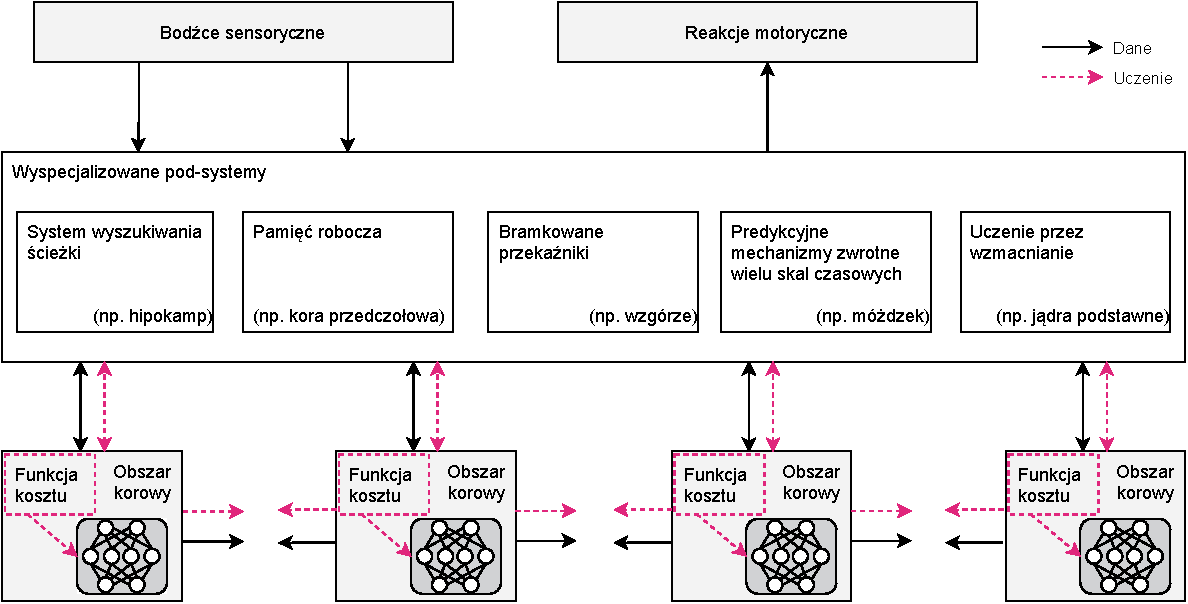
\includegraphics[width=\textwidth]{BrainLikeNeuralNetworkArchitecture.pdf}
	\caption{Proponowana struktura systemowa działania oraz uczenia się mózgu.}
	Przetłumaczona oraz zaadoptowana z \cite{marblestone2016toward}.
	Według niej mózg składa się z wielu wyspecjalizowanych pod-systemów pozwalających na wydajne wykonywanie konkretnych zadań oraz sieci neuronalnych uczonych przy użyciu funkcji kosztu zmiennych względem obszaru i w czasie.
	Wyspecjalizowane struktury znajdują się przede wszystkich w starszych ewolucyjnie częściach mózgu oraz posiadają również funkcje organizacyjno-sterujące.
	Zbiór wielu wielokrotnie trenowalnych sieci znajduje się głównie w najmłodszej ewolucyjne korze czołowej.
	Na funkcje kosztu używane przy ich trenowaniu wpływ mają struktury wyspecjalizowane oraz inne, wcześniej wytrenowane sieci.
	\label{fig:structure-with-specialized-systems}
\end{figure}

Z istotniejszych pod-systemów obecnych w mózgu można wyróżnić przede wszystkim:

\begin{itemize}
	\item \emph{Struktury pamięciowe różnego rodzaju}.
	      Są to centralne systemy dla wszelkich systemów symbolicznych, obecne już od samej maszyny Turinga \cite{turing1937computable}.
	      To, że mózg posiada struktury pamięciowe jest niepodważalne, na co jednak warto zwrócić uwagę to fakt, że musi posiadać wiele rodzajów takowych.
	      Potrzebna jest pamięć długotrwała, robocza oraz bardziej wyspecjalizowane, jak adresowane zawartością (obszar CA3 w hipokampie może działać jak pamięć auto-asocjacyjna zdolna do implementacji tego typu pamięci \cite{rolls2013mechanisms}) czy inne wspomniane na początku tego rozdziału \cite{graves2014neural}.
	      Rola i obecność takich systemów jest w psychologii poznawczej badana już od dłuższego czasu \cite{baddeley2004psychology}.
	\item \emph{Struktury kierujące informacją}.
	      Takim systemem może być struktura uwagowa, również od dłuższego czasu badana w psychologii poznawczej \cite{pashler1999psychology}.
	      Pozwala na ograniczenie natłoku danych docierających do systemów przetwarzania informacji, ograniczenie ich przeładowania oraz wstępną selekcję porcji strumienia o istotnym znaczeniu dla systemu poznającego.
	      Podobnie w przypadku uczenia: pozwala na skupienie się na pojedynczym obiekcie zamiast wszystkich danych, co dodatkowo, jak można zauważyć, przypomina uczenie sieci neuronowych, która skupia się na pojedynczej instancji na raz.
	\item \emph{Ustrukturyzowana reprezentacja stanu}.
	      Takie systemy pozwalają na wydajne wykonywanie złożonych algorytmicznie zadań.
	      Mogą to być systemy kontroli hierarchicznej, planowania przestrzennego, syntaktyki hierarchicznej, programów mentalnych czy wyobraźni \cite{marblestone2016toward}.
	      Większość jest już stosunkowo dobrze poznana i jesteśmy w stanie wskazać prawdopodobne struktury je wykonujące.
	      Są także obszary dopiero badane, takie jak przedmurze, które być może bierze udział w dynamicznym łączeniu informacji z wielu modalności \cite{crick2005function}.
\end{itemize}

Poza głównymi kategoriami takich systemów może znaleźć się znacznie więcej.
Samo uczenie przez wzmacniane opisywane w \hyperref[subsec:cost-function-is-diverse]{poprzedniej hipotezie} wydaje się być takim specjalistycznym pod-systemem, najprawdopodobniej zlokalizowanym w jądrach podstawnych \cite{doya1999computations}.

Być może więc to temu modelowi działania -- z wieloma wyspecjalizowanymi pod-systemami i uniwersalnymi sieciami szkolonymi przy użyciu odpowiednio dobieranych funkcji kosztu -- mózg radzi sobie z właściwie nieograniczenie szeroką gamą problemów w sposób nieosiągalny dla nowoczesnych systemów uczenia głębokiego i maszynowego.
Co ta tym idzie, istnieje szansa, że naśladując taki postulowany model działania mózgu jesteśmy w stanie osiągnąć znacznie więcej w tych dziedzinach.

\section{W kierunku rozwoju uczenia głębokiego oraz neuronauki}

Rzeczywiste powiązanie metod uczenia maszynowego z działaniem mózgu będzie owocowało rozwojem w obu dziedzinach.
Głębokie uczenie pozwoli nam lepiej zrozumieć i symulować działanie mózgu.
W przeciwną stronę naśladowanie działania mózgu w sieciach neuronowych prawdopodobnie poskutkuje znacznie potężniejszymi, efektywniejszymi i bardziej uniwersalnymi systemami.
W końcu narząd ten rozwijał się przez miliony lat i możemy spodziewać się, że ma w sobie masę kruczków optymalizacyjnych dotąd nam nieznanych.

W \hyperref[subsec:brain-optimizes-cost-function]{sekcji \ref*{subsec:brain-optimizes-cost-function}} zostały opisane uzasadnione biologiczne implementacje propagacji wstecznej, metody gradientu prostego lub innych możliwości przeprowadzania optymalizacji funkcji kosztu.
Nie podlega wątpliwości, że jeśli faktycznie mózg w taki sposób operuje, to robi to bardzo efektywnie.
Istnieje szansa, że rzeczywisty sposób jej implementacji okaże się także znacznie lepszy od naszych aktualnych rozwiązań przy sztucznych sieciach neuronowych.

Dotychczasowo większość największych osiągnięć uczenia maszynowego opierała się na bezpośredniej optymalizacji jednego zadania z użyciem pojedynczej funkcji kosztu.
Jednak nowe podejścia często starające się generalizować uczenie.
ImageNet to głęboka sieć neuronowa używana do \emph{uczenia transferowanego} (\emph{transfer learning}) -- to znaczy model jest najpierw uczony na potężnej bazie obrazków z przyciętą ostatnią warstwą.
Pozwala to na ``nałożenie'' później kolejnych warstw, które z kolei są trenowane pod specyficzne zadania, a zgeneralizowana wcześniej w ogromnym modelu podstawowym zdolność do wyodrębniania cech znacznie przyspiesza i upraszcza proces uczenia nowych warstw.
Jak pokazują rzeczywiste przykłady wykorzystania takiego systemu \cite{marmanis2015deep}, podejście okazuje się bardzo efektywne w działaniu.
Przypomina ono także opisywaną \hyperref[subsec:cost-function-is-diverse]{sekcji \ref*{subsec:cost-function-is-diverse}} zmienność funkcji kosztu w czasie.
Jeśli poznamy dokładnie sposoby dobierania odpowiednich funkcji względem obszaru i zadania oraz jej zmienność w czasie w działaniu mózgu, będziemy mogli przełożyć podobne techniki do głębokich sieci neuronowych, co podobnie jak przy prostym (w porównaniu do działania mózgu) uczeniu transferowanym powinno znacznie popchnąć dziedzinę do przodu.

Uczenie głębokie dopiero niedawno zaczęło wykorzystywać wyspecjalizowane systemy, jak te z pamięcią adresowaną lokacją czy zawartością \cite{graves2014neural}.
Niewykluczone, że są one kluczowe przy systemach uniwersalnych, czy może nawet generalnej sztucznej inteligencji.
W mózgu z kolei obecność takich wyspecjalizowanych regionów jest dość powszechnie przyjęta.
Niewykluczone, że inspirowanie się neuronauką w tym zakresie pozwoli na tworzenie systemów potrafiących wykonywać zadania znacznie bardziej złożone niż dzisiejsze najlepsze sieci.
Niektórzy badaczy argumentują, że właśnie takie podejście jest kluczem do budowy maszyn ``myślących'' tak, jak robią to ludzie \cite{lake2017building}.

Trzeba również zaznaczyć, że powiązania opisane w tym rozdziale są na razie tylko hipotezami.
Są one jednak empirycznie testowalne.

Jeśli mózg rzeczywiście optymalizuje funkcję kosztu i uda nam się ją poprawnie odgadnąć, finalny stan mózgowy powinien być bliski jej optimum.
Można później porównać pola recepcyjne optymalizowane w symulacji z tymi zmierzonymi w mózgu za pomocą badania fMRI.
Istnieją techniki, które pozwalają na wykonanie tego typu pomiarów i porównań \cite{dumoulin2008population}.
Innym sposobem mogą być wprowadzanie zakłóceń do struktury mózgowej, na przykład poprzez zmianę połączeń synaptycznych.
Efekt odpowiednio drobna zmiana powinna zostać ``wycofana'', system powinien wrócić do lokalnego minimum funkcji kosztu.

Udowodnienie drugiej hipotezy jest znacznie trudniejsze.
Przede wszystkich ważne jest rozwinięcie i udoskonalnie wszelkich mapowań mózgu, zarówno funkcjonalnych, jak i strukturalnych.
Można by było się spodziewać, że dla każdej funkcji kosztu obecne będą odmienne typy neuronów czy chociażby samych połączeń synaptycznych.

W końcu, jeśli założymy prawdziwość hipotezy trzeciej, że wiele różnych struktur bierze wspólnie udział w działaniach poznawczych czy obliczeniach, to zrozumienie funkcji przetwarzania danych każdego z obszarów będzie prowadzić do umożliwienia przewidywania mierzalnych zasad plastyczności \cite{marblestone2016toward}.


% Add the Bibliography to the contents page
\addcontentsline{toc}{chapter}{Bibliografia}
% Use a bibtex bibliography file refs.bib
\bibliography{refs}
% Use the plain bibliography style ordered by citation
\bibliographystyle{unsrt}

\end{document}
